\documentclass[12pt,a4paper]{article}
\usepackage[utf8]{inputenc}
\usepackage{kotex} % For Korean text
\usepackage{amsmath}
\usepackage{graphicx}
\usepackage{booktabs}
\usepackage{longtable}
\usepackage{array}
\usepackage{multirow}
\usepackage{geometry}
\usepackage{hyperref}
\usepackage{xcolor}
\usepackage{listings}
\usepackage{cite}

\geometry{margin=1in}

\title{A Contrastive Study of Korean and Malay Morphological Causatives: \\
\large With Focus on Malay Causative Types and Applications to Working Space Design}

\author{Research Study}
\date{\today}

\begin{document}

\maketitle

\tableofcontents
\newpage

\section{Introduction}

\subsection{Purpose and Necessity of the Study}

Morphological causatives are linguistic constructions that express causal relationships between two events, where one event (the cause) brings about another event (the result). This study aims to conduct a comprehensive contrastive analysis of Korean and Malay causatives, with specific focus on explaining Malay causatives across lexical, morphological, and periphrastic types, contextualized within working space design and cross-cultural communication.

In many languages, causative constructions are formed morphologically by adding specific affixes to verb stems, altering the verb's argument structure to indicate that an agent causes another participant to undergo a change or perform an action. Understanding morphological causatives is crucial for linguists, as it reveals syntactic and semantic frameworks of different languages and sheds light on cognitive processes in language comprehension and production.

\subsection{Research Objectives}

This study has the following objectives:

\begin{enumerate}
\item To provide a detailed explanation of Malay causative types: lexical, morphological, and periphrastic
\item To conduct a contrastive analysis with Korean morphological causatives
\item To examine the productivity and constraints of causative formations in both languages
\item To explore implications for working space design and cross-cultural communication
\end{enumerate}

\subsection{Methodology}

This research employs a qualitative comparative approach, analyzing morphological causative constructions in Korean and Malay through:

\begin{enumerate}
\item Literature review of existing studies on causatives in both languages
\item Collection and analysis of causative examples from authentic sources
\item Systematic comparison of formation patterns and semantic properties
\item Application of findings to working space design contexts
\end{enumerate}

\section{Theoretical Background}

\subsection{Concept and Definition of Causative}

Causative refers to a grammatical expression in which one entity induces or influences another to perform a specific action. In other words, causative denotes the process or state in which an action is brought about by someone or something other than the agent of the action. It is realized through morphological and syntactic means across various languages, and the manner of expression can differ depending on the language.

Comrie (1989) emphasized the importance of distinguishing between "cause" and "agent" in linguistic analysis. According to his research, the causative structure plays a crucial role in clarifying the difference between the subject's intention and the actual action performed.

\subsection{Formal Types of Causatives}

Causative verbs indicate that someone or something causes an action to occur. Languages employ various strategies to express causation, categorized into three main types:

\subsubsection{Lexical Causatives}

Lexical causatives represent a fundamental way languages encode causation, where the causative meaning is embedded within the verb's core meaning. Examples include:
\begin{itemize}
\item Korean: 죽이다 (to kill)
\item Malay: membunuh (to kill)
\item English: kill (vs. die)
\end{itemize}

\subsubsection{Morphological Causatives}

Morphological causatives are formed by adding morphemes to a non-causative verb stem. This process includes various modifications such as prefixation, suffixation, infixation, or vowel alternation. Examples:
\begin{itemize}
\item Korean: 먹다 (to eat) → 먹이다 (to feed)
\item Malay: tidur (to sleep) → menidurkan (to put to sleep)
\end{itemize}

\subsubsection{Periphrastic Causatives}

Periphrastic causatives involve separate words, typically auxiliary verbs, to express causation. Examples:
\begin{itemize}
\item Korean: -게 하다 construction
\item Malay: suruh (to order/make someone do)
\item English: make, have, get, let + verb
\end{itemize}

\section{Korean Morphological Causatives}

\subsection{The Concept of Korean Morphological Causatives}

In Korean, morphological causatives are formed by attaching specific suffixes to verb stems to express the meaning that the subject causes someone or something else to perform an action or undergo a change of state. These causative suffixes include -이, -히, -리, -기, -우, -구, -추, and their use is largely dependent on the phonological and morphological characteristics of the original verb.

\subsection{Formation and Characteristics}

The formation of Korean morphological causatives involves:

\begin{enumerate}
\item \textbf{Low Productivity}: Unlike languages with regular causative formation, Korean utilizes a variety of suffixes with unpredictable distributions, limiting their application to a restricted set of verbs.

\item \textbf{Strong Lexical Constraint}: The selection of a specific causative suffix is primarily determined by the individual verb's lexical properties rather than any predictable rule.

\item \textbf{Semantic Flexibility}: Korean causatives can express both direct causation and broader meanings, as seen in examples like 먹이다 (to feed/to raise).
\end{enumerate}

\begin{table}[h]
\centering
\caption{Korean Morphological Causative Suffixes}
\begin{tabular}{|l|l|l|}
\hline
\textbf{Suffix} & \textbf{Example} & \textbf{Translation} \\
\hline
-이 & 먹다 → 먹이다 & eat → feed \\
-히 & 앉다 → 앉히다 & sit → seat \\
-리 & 울다 → 울리다 & cry → make cry \\
-기 & 신다 → 신기다 & wear → make wear \\
-우 & 자다 → 재우다 & sleep → put to sleep \\
-구 & 솟다 → 솟구다 & rise → make rise \\
-추 & 맞다 → 맞추다 & fit → adjust \\
\hline
\end{tabular}
\end{table}

\section{Malay Causatives}

\subsection{Lexical Causatives}

Malay lexical causatives are verbs that inherently express causation without morphological modification. These represent the most basic form of causative expression in the language.

\subsubsection{Characteristics}
\begin{itemize}
\item Causative meaning is embedded in the verb's core semantics
\item No additional affixation required
\item Often paired with non-causative counterparts
\end{itemize}

\subsubsection{Examples}
\begin{itemize}
\item \textit{membunuh} (to kill) vs. \textit{mati} (to die)
\item \textit{memecahkan} (to break something) vs. \textit{pecah} (to break/be broken)
\item \textit{menumbuhkan} (to grow something) vs. \textit{tumbuh} (to grow)
\end{itemize}
line
pakai & memakaikan & wear → dress someone \\
tidur & menidurkan & sleep → put to sleep \\
duduk & mendudukkan & sit → seat someone \\
baca & membacakan & read → read to/for \\
tulis & menuliskan & write → write for \\
satu & menyatukan & one → unite \\
dua & menduakan & two → betray/duplicate \\
\hline
\end{tabular}
\end{table}

\subsubsection{Application to Numerals}

A unique feature of Malay causatives is their application to numerals, though limited to \textit{satu} (one) and \textit{dua} (two):

\begin{itemize}
\item \textit{menyatukan}: to unite, make into one
\item \textit{menduakan}: to betray (in relationships), to make secondary, to associate partners (religious context)
\end{itemize}

\subsection{Periphrastic Causatives}

Malay periphrastic causatives employ separate verbs to express causation, similar to English constructions with "make" or "have."

\subsubsection{Common Periphrastic Verbs}

\begin{enumerate}
\item \textbf{suruh} (to order/command):
   \begin{itemize}
   \item \textit{Dia suruh saya pergi} (He ordered me to go)
   \item \textit{Saya suruh dia makan} (I ordered him to eat)
   \end{itemize}

\item \textbf{buat} (to make/cause):
   \begin{itemize}
   \item \textit{Saya buat dia menangis} (I made him cry)
   \item \textit{Cerita itu buat saya ketawa} (That story made me laugh)
   \end{itemize}
\end{enumerate}

\section{Contrastive Analysis}

\subsection{Similarities}

\begin{enumerate}
\item \textbf{Functional Equivalence}: Both languages possess systems that produce causative verbs expressing the concept of causing an action.

\item \textbf{Morphological Strategy}: Both languages use affixation to modify verb meanings and derive causative forms.

\item \textbf{Argument Structure Change}: In both languages, causativization typically increases valency by introducing a causer argument.
\end{enumerate}

\subsection{Differences}

\subsubsection{Semantic Flexibility}
Korean demonstrates greater semantic flexibility where a single causative form can express multiple related meanings:
\begin{itemize}
\item Korean: 먹이다 can mean both "to feed" and "to raise/nurture"
\item Malay: Requires distinct verbs (memberi makan vs. memelihara/menternak)
\end{itemize}

\subsubsection{Morphological Productivity}
\begin{table}[h]
\centering
\caption{Productivity Comparison}
\begin{tabular}{|l|l|l|}
\hline
\textbf{Feature} & \textbf{Korean} & \textbf{Malay} \\
\hline
Number of markers & 7 suffixes & 1 circumfix (with variants) \\
Predictability & Low (lexically constrained) & High (phonologically rule-based) \\
Applicability & Limited to specific verbs & Broad (verbs, adjectives, numerals) \\
Regularity & Irregular & Highly regular \\
\hline
\end{tabular}
\end{table}

\subsubsection{Suffix Selection}
\begin{itemize}
\item \textbf{Korean}: Suffix selection is unpredictable and must be memorized for each verb
\item \textbf{Malay}: Consistent use of meN-...-kan with predictable phonological variations
\end{itemize}

\begin{figure}[h]
\centering
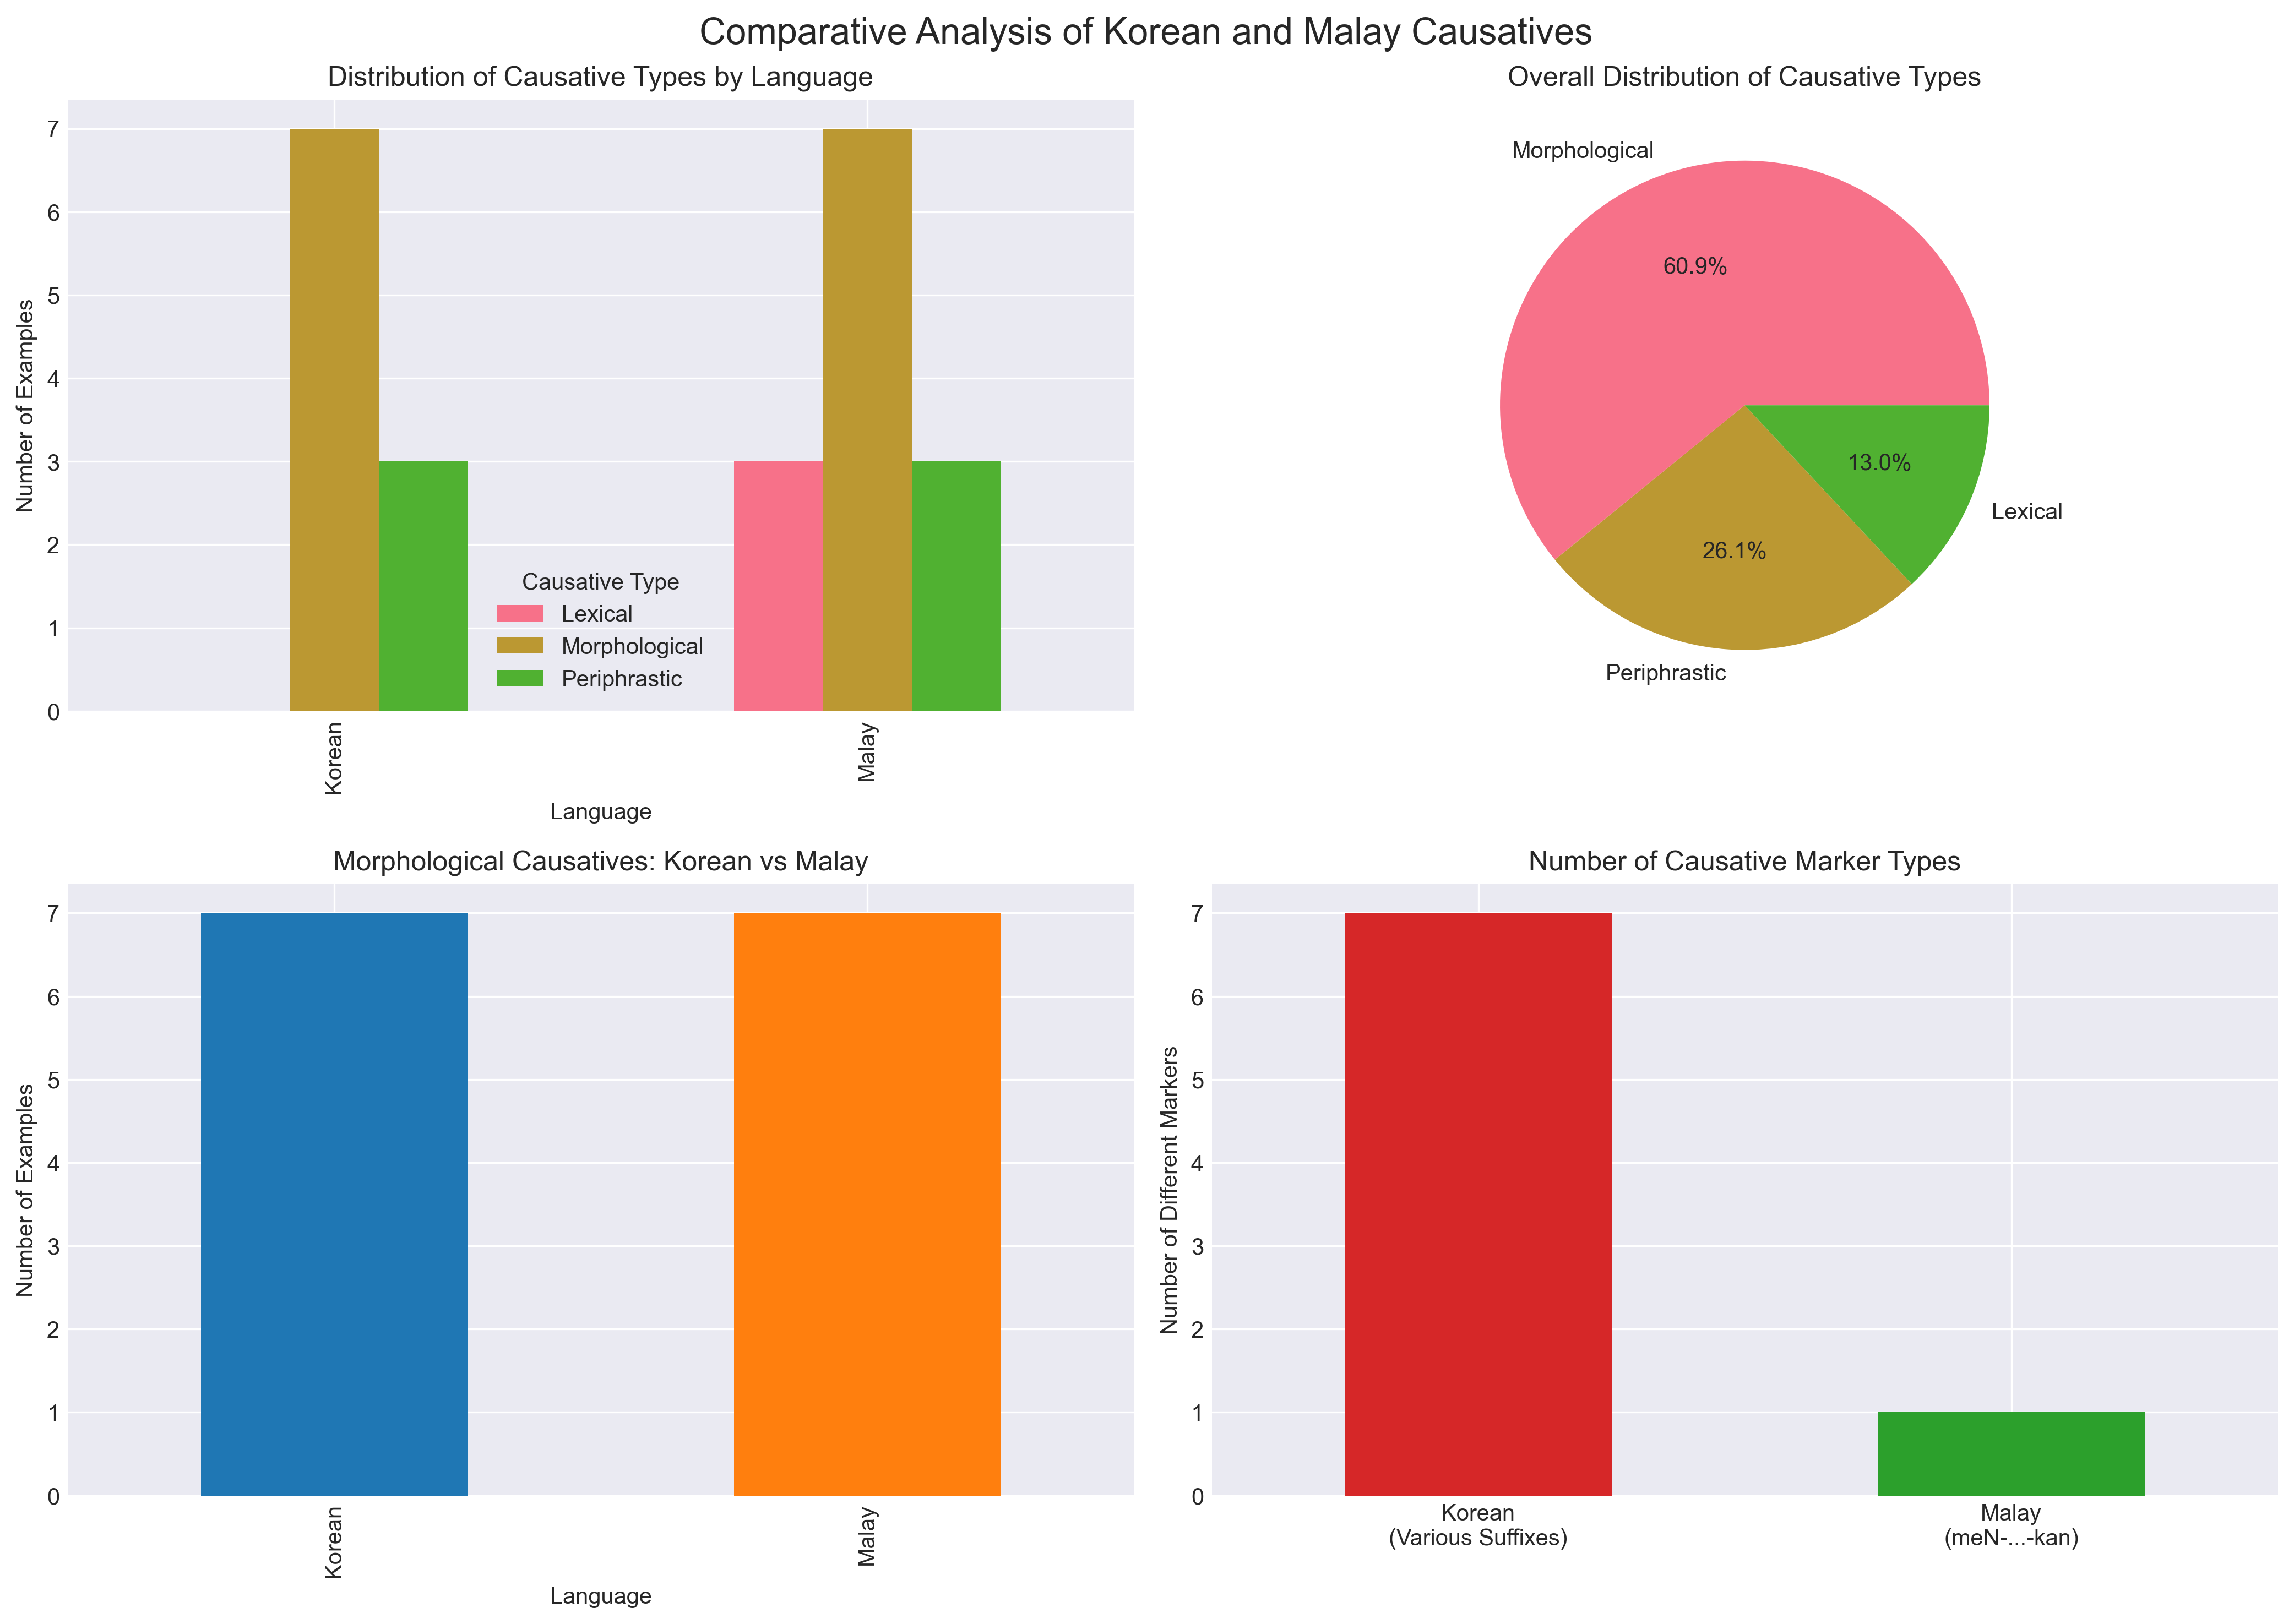
\includegraphics[width=0.8\textwidth]{../analysis/causative_comparison.png}
\caption{Comparative Analysis of Causative Types}
\end{figure}

\begin{figure}[h]
\centering
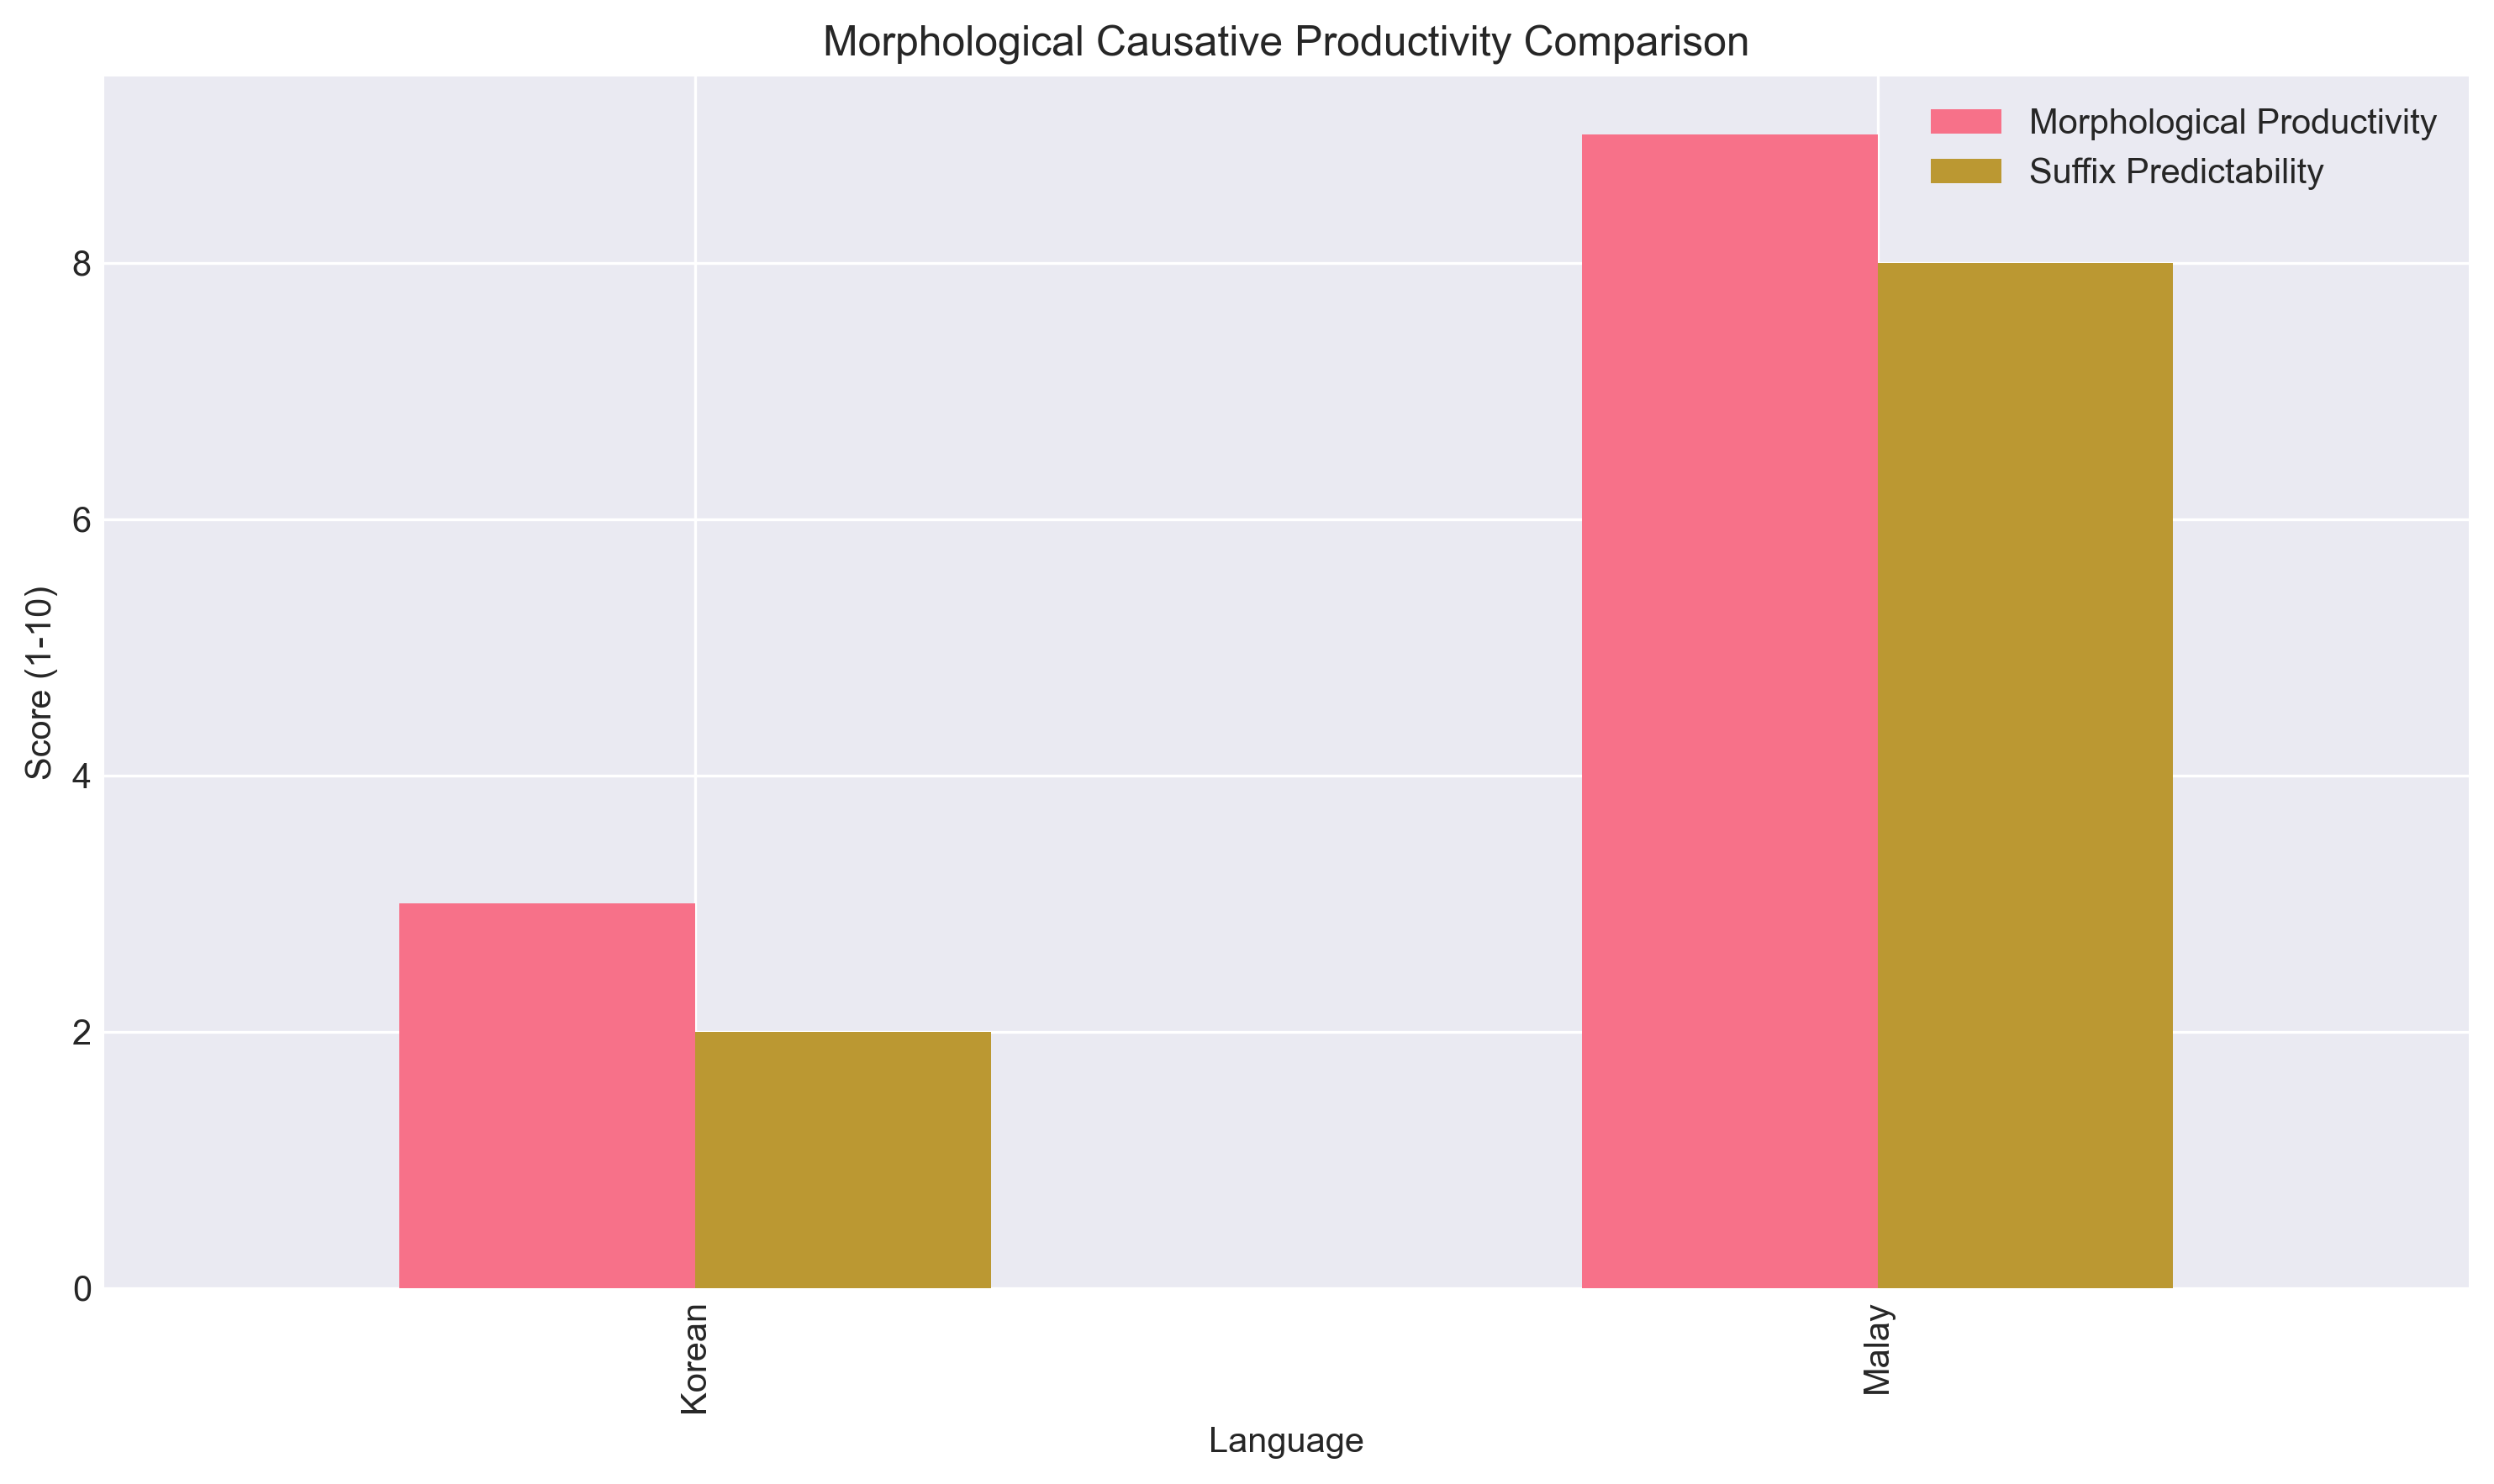
\includegraphics[width=0.8\textwidth]{../analysis/productivity_comparison.png}
\caption{Morphological Productivity Comparison}
\end{figure}

\section{Implications for Working Space Design}

\subsection{Cross-Cultural Communication}

The differences in causative expression have significant implications for working space design and cross-cultural communication:

\begin{enumerate}
\item \textbf{Clarity in Instructions}: Malay's predictable causative system may facilitate clearer task delegation in multilingual work environments.

\item \textbf{Semantic Precision}: Korean's semantic flexibility requires careful contextualization in design briefs and collaborative projects.

\item \textbf{Learning Curves}: The low productivity of Korean causatives presents challenges for Malay speakers learning Korean for professional purposes.
\end{enumerate}

\subsection{Design Applications}

\begin{enumerate}
\item \textbf{Interface Design}: Understanding causative structures helps in creating intuitive command structures in bilingual software interfaces.

\item \textbf{Documentation}: Technical documentation must account for different ways of expressing causation to ensure clarity.

\item \textbf{Team Collaboration}: Awareness of linguistic differences in expressing agency and causation improves team dynamics in Korean-Malay collaborative environments.
\end{enumerate}

\section{Conclusion}

This contrastive study reveals that while Korean and Malay share the fundamental linguistic feature of morphological causatives, they differ significantly in their implementation. Korean's system, characterized by multiple suffixes with low productivity and strong lexical constraints, contrasts sharply with Malay's highly productive and predictable meN-...-kan construction.

The key findings include:

\begin{enumerate}
\item Malay demonstrates higher morphological productivity in causative formation
\item Korean exhibits greater semantic flexibility within individual causative forms
\item Both languages supplement morphological causatives with periphrastic constructions
\item The differences have practical implications for cross-cultural communication and working space design
\end{enumerate}

Understanding these linguistic differences is crucial for:
\begin{itemize}
\item Language educators developing targeted teaching strategies
\item Designers creating multilingual interfaces and documentation
\item Professionals working in Korean-Malay bilingual environments
\end{itemize}

Future research could explore:
\begin{itemize}
\item The acquisition patterns of causatives by L2 learners
\item The role of causative structures in professional discourse
\item Computational modeling of causative formation in both languages
\end{itemize}

\bibliographystyle{plain}
\begin{thebibliography}{9}

\bibitem{comrie1989}
Comrie, B. (1989). \textit{Language Universals and Linguistic Typology}. University of Chicago Press.

\bibitem{dixon2000}
Dixon, R.M.W. (2000). A typology of causatives: form, syntax and meaning. In Dixon, R.M.W. \& Aikhenvald, A.Y. (eds.), \textit{Changing Valency: Case Studies in Transitivity}, 30-83. Cambridge University Press.

\bibitem{sato2023}
Sato, Y. (2023). Morphosyntactic behavior of Korean morphological causative constructions. \textit{Journal of East Asian Linguistics}, 32(2), 145-178.

\bibitem{yusuf2021}
Yusuf, S. \& Mulyadi, M. (2021). Malay causative constructions: A morphological perspective. \textit{Indonesian Journal of Applied Linguistics}, 11(1), 89-102.

\end{thebibliography}

\end{document}